\documentclass{article}
\usepackage{tikz}
\usetikzlibrary{calc}

\begin{document}

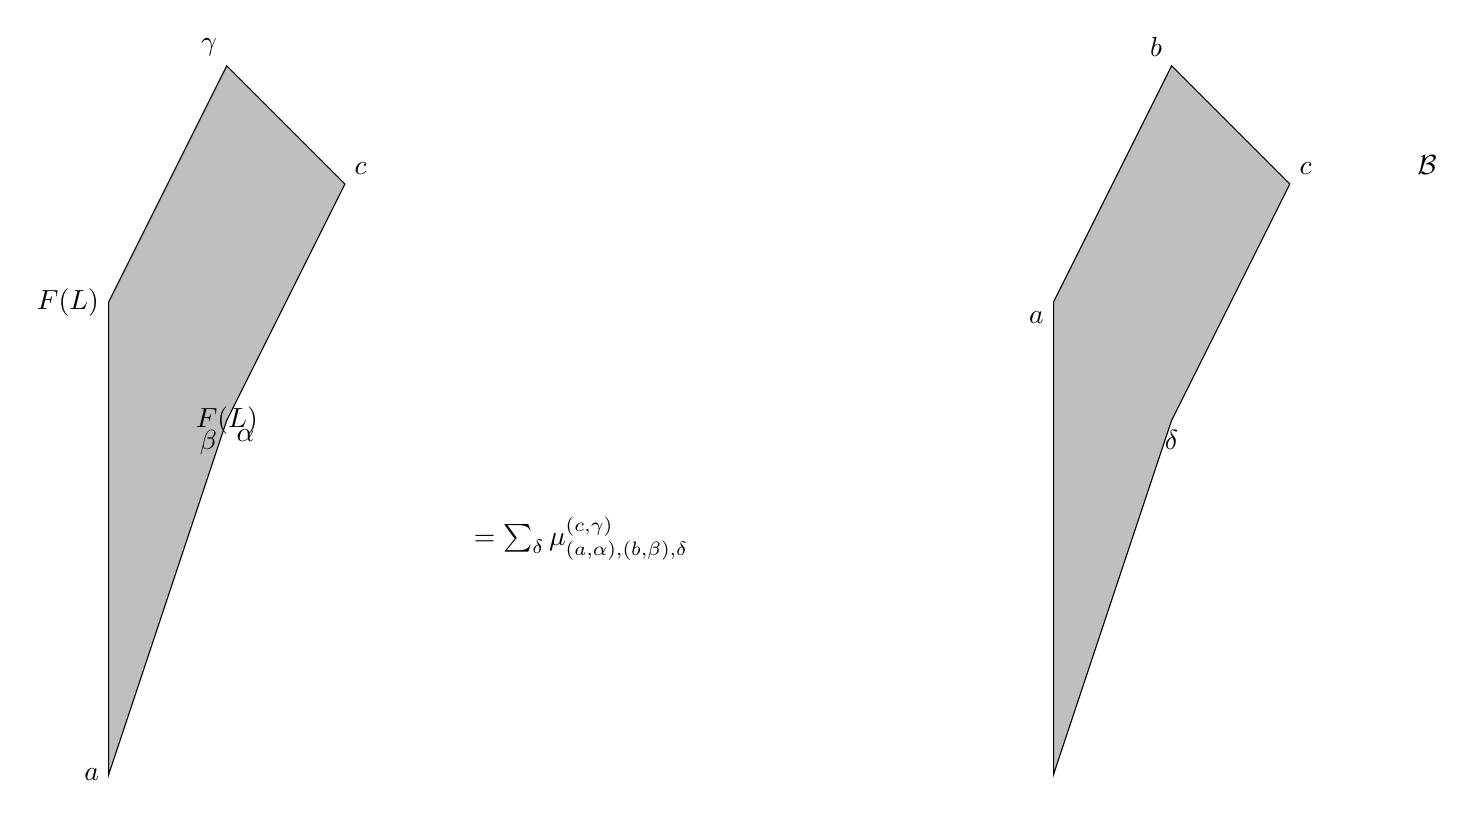
\begin{tikzpicture}[scale=1.5]
    % Draw the first polygon and labels
    \filldraw[fill=gray!50, draw=black] (-2, -2) -- (-1, 1) -- (0, 3) -- (-1, 4) -- (-2, 2) -- cycle;
    \node at (-1, 1) {$F(L)$};
    \node at (-2, -2) [left]{$a$};
    \node at (-2, 2) [left]{$F(L)$};
    \node at (0, 3) [above right]{$c$};
    \node at (-1, 4) [above left]{$\gamma$};
    \node at (-1, 1) [below right]{$\alpha$};
    \node at (-1, 1) [below left]{$\beta$};
    
    % Draw the second polygon and labels
    \filldraw[fill=gray!50, draw=black] (6, -2) -- (7, 1) -- (8, 3) -- (7, 4) -- (6, 2) -- cycle;
    \node at (7, 1) [below]{$\delta$};
    \node at (6, 2) [below left]{$a$};
    \node at (8, 3) [above right]{$c$};
    \node at (7, 4) [above left]{$b$};
    
    % Draw the text in the middle
    \node at (2, 0) {$= \sum_{\delta} \mu^{(c,\gamma)}_{(a,\alpha),(b,\beta),\delta}$};
    
    % Label the polygon
    \node at (9, 3) [above right]{$\mathcal{B}$};
\end{tikzpicture}

\end{document}